\documentclass{article}
\usepackage{graphicx}
\usepackage{amsmath}
\usepackage{bm}
\usepackage{mathptmx}
\usepackage[parfill]{parskip}

\usepackage{graphicx}
\usepackage{amsmath, amssymb, amsthm}
\usepackage{epsf}
\usepackage{bm}
\usepackage[parfill]{parskip}
\usepackage{mathptmx}
\usepackage{geometry}
\usepackage{fancyhdr}

\newcommand{\mc}[1]{\mathcal{#1}}
\newcommand{\mbf}[1]{\mathbf{#1}}
\def\E{\mathbb{E}}


\renewcommand{\thesection}{\Roman{section}}
\renewcommand{\thesubsection}{\Alph{subsection}}

\newcommand{\params_J}{100}
\newcommand{\params_J}{100}
\newcommand{\params_edu_types}{['H', 'L']}
\newcommand{\params_race_types}{['White', 'Black']}
\newcommand{\params_gamma_HH}{-0.2}
\newcommand{\params_gamma_HL}{0.5}
\newcommand{\params_gamma_LL}{-0.5}
\newcommand{\params_gamma_LH}{0.7}
\newcommand{\params_alpha_HH}{0.8}
\newcommand{\params_alpha_HL}{0.1}
\newcommand{\params_alpha_LH}{0.2}
\newcommand{\params_alpha_LL}{0.7}
\newcommand{\params_iota}{0.05}
\newcommand{\params_phi}{1}
\newcommand{\params_phi_geo}{0.3}
\newcommand{\params_phi_reg}{0.4}
\newcommand{\params_phi_a}{0.5}
\newcommand{\params_zeta}{0.8}
\newcommand{\params_beta_st}{3}
\newcommand{\params_beta_st}{3}
\newcommand{\params_beta_x}{{'White': 0.3, 'Black': 0.7}}
\newcommand{\params_beta_a}{{'White': 0.3, 'Black': 0.9}}
\newcommand{\params_beta_w}{{'White': 0.9, 'Black': 0.2}}
\newcommand{\params_H}{{'Black': {'N': 20}, 'White': {'N': 80}}}
\newcommand{\params_L}{{'Black': {'N': 180}, 'White': {'N': 20}}}
\newcommand{\params_Z_H}{{'mu': 0, 'sigma': 0.5}}
\newcommand{\params_Z_L}{{'mu': 0, 'sigma': 0.5}}
\newcommand{\params_x_geo}{{'mu': 0, 'sigma': 0.5}}
\newcommand{\params_x_reg}{{'mu': 0, 'sigma': 0.5}}
\newcommand{\params_CC}{{'mu': 0, 'sigma': 0.1}}
\newcommand{\params_x}{{'mu': 0, 'sigma': 0.1}}
\newcommand{\params_epsilon_H}{{'mu': 2, 'sigma': 0.1}}
\newcommand{\params_epsilon_L}{{'mu': 1, 'sigma': 0.1}}
\newcommand{\params_epsilon_a}{{'mu': 0, 'sigma': 0.1}}

\newcommand{\paramsestbetawWhite}{0.8995}
\newcommand{\paramsestbetaaWhite}{0.3019}
\newcommand{\paramsestbetawBlack}{0.1979}
\newcommand{\paramsestbetaaBlack}{0.9022}
\newcommand{\paramsestbetast}{3.0096}
\newcommand{\paramsestalphaHH}{0.8046}
\newcommand{\paramsestalphaHL}{0.0992}
\newcommand{\paramsestgammaHH}{-0.2117}
\newcommand{\paramsestgammaHL}{0.5241}
\newcommand{\paramsestalphaLH}{0.1916}
\newcommand{\paramsestalphaLL}{0.7019}
\newcommand{\paramsestgammaLH}{0.7264}
\newcommand{\paramsestgammaLL}{-0.5337}
\newcommand{\paramsestiota}{0.0501}
\newcommand{\paramsestphi}{0.9971}
\newcommand{\paramsestphigeo}{0.3007}
\newcommand{\paramsestphireg}{0.4012}
\newcommand{\paramsestphia}{0.4983}


\title{14.273 IO Problem Set 2}
\author{Benjamin Wittenbrink, Jack Kelly, and Veronicá Bäcker-Peral}

\begin{document}

\maketitle

\section{Production Function Estimation}

This problem uses data from the NBER Working Paper Grilliches and Mairesse (1995) (henceforth, GM), and builds on previous problem sets by Aviv Nevo, Allan Collard-
Wexler, and Jan DeLoecker. The dataset (\texttt{gmData.csv}) contains nine variables: 
\begin{itemize}
\item \texttt{index}: Firm ID
\item \texttt{sic3}: 3-digit SIC code
\item \texttt{yr}: Year
\item \texttt{ldsal}: Log deflated sales
\item \texttt{lemp}: Log employment
\item \texttt{ldnpt}: Log deflated capital 
\item \texttt{ldrst}: Log deflated R\&D capital
\item \texttt{ldrnd}: Log deflated R\&D
\item \texttt{ldinv}: Log deflated investment
\end{itemize}
For additional details on the data, see Hall (1990). 

We are interested in estimating the following production function:
\begin{equation}\label{p1_prod_fn}
y_{it} = \beta_1 \ell_{it} + \beta_2 k_{it} + \beta_3 r_{it} + \delta_t + \gamma_{ts} + \omega_{it} + \varepsilon_{it},
\end{equation}
where $\delta_t$ denotes year fixed effects and $ \gamma_{ts}$ denotes year fixed effects for industry 357. 

Answer the following questions:

\subsection{Reproducing GM Results}
\begin{enumerate}

\item Reproduce Columns 1–4 of Table 3 in GM by estimating different versions of
Equation (\ref{p1_prod_fn}).

\begin{answer}

We reproduced the results in GM in Table \ref{tab:gm_rep}.

\begin{table}[H]
\centering
\caption{Replication of GM}
\label{tab:gm_rep}
\begin{tabular}{lcccc}
\toprule
& (1) & (2) & (3) & (4) \\ 
 & Balanced, Total & Balanced, Within & Full, Total & Full, Total (+ Investment) \\
\midrule
Log employment & 0.496 & 0.685 & 0.578 & 0.551 \\
 & (0.022) & (0.030) & (0.013) & (0.013) \\
Log capital & 0.460 & 0.180 & 0.372 & 0.298 \\
 & (0.014) & (0.027) & (0.009) & (0.012) \\
Log R\&D capital & 0.034 & 0.099 & 0.038 & 0.027 \\
 & (0.015) & (0.027) & (0.007) & (0.007) \\
Log investment &  &  &  & 0.110 \\
 &  &  &  & (0.011) \\
 \midrule 
N & 856 & 856 & 2,971 & 2,971 \\
$R^2$ & 0.968 & 0.994 & 0.962 & 0.963 \\
\bottomrule
\end{tabular}
\end{table}

\end{answer}


\item Compare the estimates in Column 3 and Column 1. What insights do you
draw from the differences?

\begin{answer}
The estimated effect of employment relative to capital is larger in the full dataset. This tells us that firms that were created after 1973 or closed before 1988 had higher employment shares than firms that were in existence over the full period.
\end{answer}


\item Compare these results with Column 1 of Table VI in Olley and Pakes (1996).
What do you learn from the comparison?

\begin{answer}
In Table VI of Olley and Pakes (1996), the authors estimate that the labor share of output is much larger than what GM estimate. This suggests that endogeneity between the choice of labor, investment and productivity shocks bias downward the observed relationship between employment and output.
\end{answer}

\end{enumerate}

\subsection{Dynamic Panel Model}
Following the dynamic panel model in Ackberg, Caves, and Frazer (2015) (henceforth, ACF) in Section 4.3.3:

\begin{enumerate}
\item Derive the $\rho$–dfferenced version of Equation (\ref{p1_prod_fn}).

\begin{answer}

We calculate the $\rho$-differenced version as $y_{it} - \rho y_{it}$. Applying this to our setting we obtain 
\begin{align*}
    y_{it} - \rho  y_{it-1}
    & = \beta_1 (\ell_{it} - \rho \ell_{it-1}) + \beta_2 (k_{it} - \rho k_{it-1}) \\ 
    &\quad \quad + \beta_3 (r_{it}  - \rho r_{it-1}) 
    + (\delta_t - \rho \delta_{t-1}) \\ 
    &\quad\quad + (\gamma_{ts} - \rho \gamma_{t-1, s}) + \xi_{it} + (\varepsilon_{it}-\rho\varepsilon_{it-1}),
\end{align*}
where $\omega_{it} = \rho \omega_{it-1} + \xi_{it}$ under the assumption that $\omega_{it}$ follows an AR(1) process. 


\end{answer}



\item State the analog of ACF’s assumptions in this context. 

\begin{answer}

ACF assume for their context that: 
\begin{enumerate}
    \item $\varepsilon_{it}$ is iid over time and uncorrected with $I_{it}$; 
    \item $\omega_{it}$ is correlated with $k_{it}$ and $\ell_{it}$ $\forall t$; 
    \item $\xi_{it}$ is uncorrelated with $I_{it-1}$ (i.e., all input choices before $t$). 
\end{enumerate}

%Similarly, in this context, we also assume that $\varepsilon_{it}$ is iid over time and uncorrelated with the information set $I_{it}$.
Our assumptions in this context are similar. ...  We also impose that $\xi_{it}$ is uncorrelated with all input choices before $t$ (i.e., employment, capital, and R \& D capital).

\end{answer}


\item Write the corresponding version of ACF’s Equation (34).


\begin{answer}

In ACF, they estimate the model using the moment condition: 
\[
E[\xi_{it} + (\varepsilon_{it} - \rho \varepsilon_{it-1}) \mid I_{it-1}] =0.
\]
In our context, this is given as 
\begin{align*}
E[\xi_{it} + (\varepsilon_{it} - \rho \varepsilon_{it-1}) \mid I_{it-1}] &= 
E[(y_{it} - \rho  y_{it-1}) - \beta_1 (\ell_{it} - \rho \ell_{it-1}) \\
&\quad \quad - \beta_2 (k_{it} - \rho k_{it-1}) - \beta_3 (r_{it}  - \rho r_{it-1}) \\
&\quad \quad - (\delta_t - \rho \delta_{t-1})-(\gamma_{ts} - \rho \gamma_{t-1, s})
\mid I_{it-1}] \\
&= 0.
\end{align*}


\end{answer}




\item List the set of valid instruments based on your stated assumptions.


\begin{answer}

Any variable that was chosen in period $t-1$ is a valid instrument. Thus, period $t$ capital and R \& D capital (assuming dynamic) are valid. Additionally, period $t-1$ employment is valid. 

\end{answer}


\item Estimate the dynamic panel model using GMM and compare the results with
those from Equation (\ref{p1_prod_fn}).


\end{enumerate}


\subsection{ACF First Stage Moments}

\begin{enumerate}

\item Write down the first-stage ACF moment condition.


\begin{answer}
Given the monotonicity assumptions, we can invert the production function and write, $\omega_{it}=f_t^{-1}(k_{it},\ell_{it},r_{it},i_{it})$. Define,
$$\Phi_t (k_{it},\ell_{it},r_{it},i_{it}) = \beta_1 \ell_{it} + \beta_2 k_{it} + \beta_3 r_{it} + f_t^{-1}(k_{it},\ell_{it},r_{it},i_{it})$$
which includes all dependence on capital and labor. Then, the first stage moment condition is,
$$E[y_{it} - \Phi_t(k_{it},\ell_{it},r_{it},i_{it})|\delta_t,\lambda_{ts},I_t]=0$$
In words, this says that the transitory shock $\epsilon_{it}$ -- which can be written as the production function purged of any dependence on capital, labor -- is ``unexpected": orthogonal to all information available at time $t$.
\end{answer}

\item Estimate the first-stage ACF regression using \texttt{ldinv} as the measure of investment.

\begin{answer}
See attached code. In the first stage, we flexibly estimate the function $\Phi$ using a polynomial.
\end{answer}

\end{enumerate}

\subsection{ACF Second Stage Moments:}

\begin{enumerate}
\item Write down the second-stage ACF moment condition.

\begin{answer}
We can decompose productivity shocks as, $\omega_{it} = E[\omega_{it} | \omega_{it-1}] + \xi_{it} = \rho\omega_{it-1} + \mu + \xi_{it}$, assuming that productivity follows an AR(1) process. Substituting this into the production function,
\begin{align*}
    y_{it} &= \beta_1 \ell_{it} + \beta_2 k_{it} + \beta_3 r_{it} + \delta_t + \gamma_{ts} + \rho\omega_{it-1} + \mu + \xi_{it} + \varepsilon_{it} \\
    &= \beta_1 \ell_{it} + \beta_2 k_{it} + \beta_3 r_{it} + \delta_t + \gamma_{ts} \\
    &\quad+ \rho(\Phi_{t-1}(k_{it-1}, \ell_{it-1}, r_{it-1},i_{it-1}) - \beta_1 \ell_{it-1} - \beta_2 k_{it-1} - \beta_3 r_{it-1}) + \xi_{it} + \varepsilon_{it} \\
\end{align*}
where the constant $\mu$ is absorbed into the year fixed effects. The second stage moment condition is,
\begin{align*}
    E[\xi_{it} + \varepsilon_{it} | I_{it-1}]&=E[y_{it} - \beta_1 \ell_{it} - \beta_2 k_{it-1} - \beta_3 r_{it} + \delta_t + \gamma_{ts} \\
    &\quad -\rho(\Phi_{t-1}(k_{it-1}, \ell_{it-1}, r_{it-1},i_{it-1}) - \beta_1 \ell_{it-1} - \beta_2 k_{it-1} - \beta_3 r_{it-1})|I_{it-1}]=0
\end{align*}
Converting this into an unconditional moment restriction,
\begin{align*}
    &E[(y_{it} - \beta_1 \ell_{it} - \beta_2 k_{it-1} - \beta_3 r_{it} + \delta_t + \gamma_{ts} \\
    &\quad -\rho(\Phi_{t-1}(k_{it-1}, \ell_{it-1}, r_{it-1},i_{it-1}) - \beta_1 \ell_{it-1} - \beta_2 k_{it-1} - \beta_3 r_{it-1})) \otimes I_{it-1}]=0
\end{align*}
where 
$$I_{it-1} = \begin{bmatrix}
    1 \\
    k_{it} \\
    l_{it-1} \\
    \Phi_{t-1}
\end{bmatrix}$$

\end{answer}
\item Estimate the second-stage ACF model to recover $\beta_1, \beta_2,$ and $\beta_3$ under the assumption $\omega_{it} = \rho \omega_{i t-1} + \mu + \xi_{it}.$

 \begin{answer}
We estimate the parameters as in ACF. We iterate over the parameters $\beta_1, \beta_2, \beta_3$. For each parameter guess, we construct,
$$\hat{\lambda}_{it} = \widehat{\delta_t + \gamma_{ts} + \omega_{it}} = \hat{\Phi} - \beta_1 \ell_{it} - \beta_2 k_{it} - \beta_3 r_{it}$$
Then, a regression,
$$\hat{\lambda}_{it} = \mu + \rho \hat{\lambda}_{it-1} + \xi_{it}$$
yields an estimate of $\hat{\rho}$ and $\hat{\mu}$. The residual of this regression is $\xi_{it}$, which by assumption are orthogonal to our instruments at the true parameter values. Therefore, we can calculate our GMM moments condition,
$$E[\xi_{it}|I_{it-1}] = 0$$
Then, we can search over the $\beta_i$'s to find the parameter values that minimizes the objective function.
 \end{answer}


\item Compare these results with those from both Equation (\ref{p1_prod_fn}) and your previous
estimation.

\begin{answer}
We estimate $\rho=0.47$, $\mu=1.23$, and $\beta=(0.56, 0.41, 0.03)$. These parameters are similar to our earlier values, but our new estimate for $\rho$ is larger.
\end{answer}

\item Contrast your findings with Column 5 of GM.

\begin{answer}
Our findings are approximately similar to those in Column 5 of GM.
\end{answer}

\end{enumerate}


\subsection{ACF Moments with Survival Control}
Redo the second-stage ACF moments incorporating a survival control in the evolution of $\omega$ (i.e,. where survival depends on capital and year). Compare your new estimates with those obtained in part (4) and with Column 6 of GM.

\begin{answer}
Suppose now that productivity shocks do not follow a simple AR(1) process. Instead, 
$$\omega_{it} = \rho\omega_{it-1} + g_t(k_{it-1}) + \xi_{it}$$
Then, substituting this into the production function,
\begin{align*}
    y_{it} &= \beta_1 \ell_{it} + \beta_2 k_{it} + \beta_3 r_{it} + \delta_t + \gamma_{ts} + \rho\omega_{it-1} + g_t(k_{it-1}) + \xi_{it} + \varepsilon_{it} \\
    &= \beta_1 \ell_{it} + \beta_2 k_{it} + \beta_3 r_{it} + \delta_t + \gamma_{ts} \\
    &\quad+ \rho(\Phi_{t-1}(k_{it-1}, \ell_{it-1}, r_{it-1},i_{it-1}) - \beta_1 \ell_{it-1} - \beta_2 k_{it-1} - \beta_3 r_{it-1}) + g_t(k_{it-1}) + \xi_{it} + \varepsilon_{it} \\
\end{align*}
Then, we can choose a paramterization of $g$ and solve for these paramters in our estimation. For computational simplicity, assume a linear parameterization,
$$g_t(k_{it-1}) = \alpha k_{it-1} + \chi_t$$
Note that the $\chi_t$ will be absorbed into our other fixed effects, $\delta_t$. However, we will add an extra parameter, $\alpha$, that we will search over in GMM. With this paramterization, our estimates of $\beta$ change substantially to (0.101,0.237, 0.306), since part of the effect of capital on sales is absorbed by $\alpha$. Moreover, our $\rho$ becomes larger at around 0.76.

\end{answer}



\subsection{Mark-Up Calculation}
Calculate mark-ups using labor as a variable input (consult De Loecker and Warzynski (2012) for reference). Note that \texttt{lemp} represents the logarithm of the quantity
of employed workers (in thousands). To do this:

\begin{answer}
As in De Loecker and Warzynski (2012), we can use the above methodology to obtain the output elasticity of labor,
$$\theta_{it}^L = \hat{\beta}_1 $$
The expenditure share of labor is,
$$\alpha_{it}^L = \frac{W_{it}L_{it}}{Y_{it}}$$
Then, we estimate mark ups as,
$$\mu_{it} = \frac{\theta_{it}^L}{\alpha_{it}^L}$$
\end{answer}

\begin{enumerate}
\item Merge the industry-level wage data from \texttt{sic5811.csv}.
\item Plot both the share-weighted and unweighted time series of mark-ups. 

\begin{answer}
The markups are plotted in Figure~\ref{fig:markups}. We calculate average markups across all industries. The blue line presents the simple average markup. The orange line presents the average markup, weighted by the share of sales for that industry.

\begin{figure}[H]
    \centering
    \caption{Markups}
    \label{fig:markups}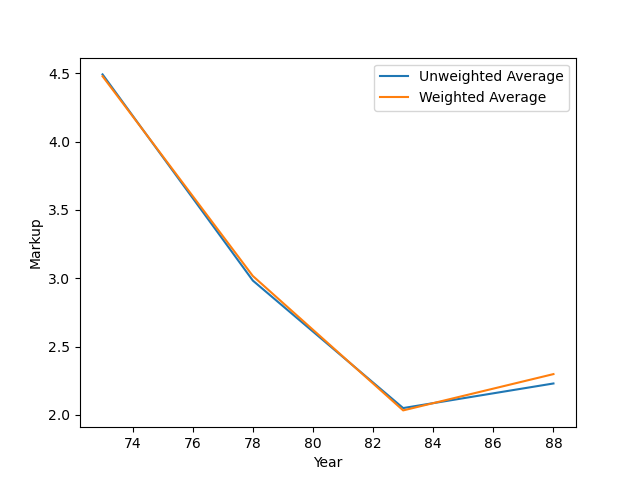
\includegraphics[width=0.5\linewidth]{Problem Set 2/markup_timeseries.png}
\end{figure}

\end{answer}


\item Comment on your findings. 

\begin{answer}
The markups are falling in the 70s and then reverse in the 80s. Note that our estimated output elasticity with respect to labor is a constant, so these results are driven entirely due to variation in labor share of sales. 
\end{answer}

\end{enumerate}

\section{Entry Model}

Consider a two-period model in which firms decide whether to enter in the first period, and only entrants earn profits in the second period.

\subsection{First Period}
\begin{itemize}
\item There are $F$ potential entrants.
\item The fixed cost of entry for firm $f$ into market $m$ is given by:
\begin{equation}
\phi_{fm} = Z_{fm} \alpha + u_{fm},
\end{equation}
where $u_{fm} \sim N (\mu, \sigma^2)$ and $Z_{fm}$ represents a firm-market characteristic.
\item Firms observe all variables in the model and enter sequentially. The firm with the lowest realized fixed cost enters first (if profitable), followed by the firm with the second lowest cost, and so on. The payoff from not entering is normalized to zero.
\end{itemize}

\subsection{Second Period}

Once entry decisions are made, firms realize their net profit (including the fixed cost) given by:

\begin{equation}
\pi_{fm} = X_m \beta - \delta \log N_m - \phi_{fm},
\end{equation}

where $N_m$ is the number of firms that entered market $m$ and $X_m$ is a market characteristic. The profit for not entering remains normalized to zero.

\subsection{Parameters}

For this problem, assume the true parameter values are:
\begin{itemize}
\item $F = 3$
\item $(\alpha, \beta, \delta) = (1, 1, 1)$
\item $(\mu, \sigma^2) = (2, 1)$
\end{itemize}

The observable characteristics are distributed as follows:
\begin{itemize}
\item $X_m \sim N (3, 1)$
\item $Z_{fm} \sim N (0, 1)$
\end{itemize}

There are $M = 100$ markets. The dataset \texttt{entryData.csv} contains data for these markets with 7 columns: $X_m$, ${Z_{fm}}{f=1}^{F}$, and the entry decisions of each firm (dummy variables in the same order as $Z{fm}$).

\subsection{Questions}

\begin{enumerate}
\item \textbf{Berry (ECMA 1992):} Suppose that $(\alpha, \beta, \delta)$ and $F$ are known. Your goal is to estimate $(\mu, \sigma^2)$ using the observable market data. Construct a maximum likelihood estimator and implement a simulated likelihood approach under the correct assumption regarding the order of entry.

\begin{answer}

We start by solving the game. 

Observe first that while the $u_{fm}$ draws are unknown to the econometrician, they are known to the firms, i.e., this is a dynamic game of complete information. 

We can therefore solve for the essentially unique Subgame Perfect Nash Equilibrium via backwards induction, ordering players by their  values of $\phi_s$. We denote the firm with the $n$th lowest fixed cost in market $m$ by $f_m^{\#n}$. The last player in the game, $\phi_{f^{\#3}_m}$, will enter only if $ \pi_{f^{\#3}_m }(N_m=3)\geq0$. If they enter, all previous firms enter, since  their fixed costs are lower. If they do not enter, then the firm with the second highest $\phi$ in a given market, $\phi_{f^{\#2}m}$, will enter only if $ \pi_{f^{\#2}m }(N=2)\geq 0$, and so on and so forth. Essential uniqueness follows from the fact that $ \pi_{f^{r}_m }(N_m=r)=0$ with probability 0 for each $r,m$, given the continuously distributed shocks and continuous profit function. 

So, to simulate the likelihood of the data we observe, we  run the following procedure  

\begin{enumerate}
\item For a given $\mu, \sigma^2$, and for each simulation draw, draw cost shocks.
\item Within each market, order firms by their $\phi_{jm}$
\item For each firm in a given market who is ranked $r$ in terms of its $\phi_{jm}$ (in ascending order) calculate $\pi_{f^{r}_m }(N=r)$
\item Find the highest $r$ firm (if any) within each market such that $\pi_{f^{r}m }(N=r) \geq 0$, and set the entry variable equal to 1 for that firm and all firms in that market ranked below $r$. 
\item 
Run this simulation 500 times and take the average entry dummy for each observation to get its simulated likelihood, \textit{prob\_enter}. Then the log likelihood for a given draw is $I\{entered\} \times \ln(prob\_enter) + (1-I\{entered\}) \times \ln (1-prob\_enter)$. We take the sum across observations to get the log likelihood. 

We minimize the negative of the log likelihood using a direct search algorithm (because of the discrete nature of the problem, gradient-based numerical optimization methods perform poorly here). The results can be found in table \ref{tab:entry_table}. 
\end{enumerate}

$\textit{}$


\end{answer}
\item \textbf{Ciliberto and Tamer (ECMA 2009):}
\begin{enumerate}
\item[(a)] Write a function \texttt{calc\_mi(mu; data)} that computes the moment inequality objective value.
\begin{answer}
The moment we minimize is 
$$
\frac{1}{M}\sum_{m\in \mathcal{M}}||\min \{P(y|X_m)-H_1((\mu,\sigma^2),X_m),0\}||_2 + ||\max \{P(y|X_m)-H_2((\mu,\sigma^2),X_m),0\}||_2
$$

where $P(y|X_m)$ is, for each market, a $2^F$ dimensional vector giving the probability of each possible entry configuration given the data, $H_1((\mu,\sigma^2),X_m)$ is the pointwise lower bound on probability of each entry configuration, and $H_2(\cdot)$ is the pointwise upper bound. In particular, $H_2$ is the probability that the entry vector is  \textit{an}  equilibrium (corresponding to an equilibrium selection mechanism in which it is always chosen when there are multiple equilibria), and $H_1$ is the probability it is the \textit{unique} equilibrium (corresponding to a selection mechanism in which it is never chosen if there are multiple equilibria).

The idea here is that at a value of $\mu$ in the identified set, we should never have a minimum probability of entry that is greater than the observed probability of entry, and likewise the max probability of entry should always weakly exceed the observed probability. The objective function penalizes such deviations and looks for the parameter value that minimizes deviations (so it corresponds to some point in the identified set).

Of course, we do not observe $P(y|X_m)$ or the $H(\cdot)$ functions. We construct them as follows:
\begin{enumerate}
\item We calculate $P(y|X_m)$ as a multinomial logit. In particular, we treat each market as an observation with covariates $X,Z_1,Z_2,Z_3$ (and a constant), and form the outcome as the entry vector we observe in the data. The multinomial logit model extends the classic logit binary choice model to multiple unordered outcomes by allowing for a different coefficient for each outcome on each covariate (i.e., $\beta_m^x$ measures how much a covariate $x$ makes outcome $m$ more likely, all else equal). One wrinkle in estimation here is that of the $2^3=8$ possible entry vectors, only 4 are observed in the data. We simply set $P(y^j|X_m)=0$ for $j$ in the set of unobserved entry vectors.

\item We calculate $H_1,H_2$ by simulation. In particular, for each simulation draw, for each guess of $\mu$ (recall that $\sigma^2$ is known now and equal to 1) we scale up a set of $FM$ draws from a standard normal appropriately (corresponding to one cost shock per firm). We then use the formula for $\phi_{fm}$ and the profit function to compute a firm's profits under each possible entry vector. Then for each possible entry vector, we check for whether it is a Nash equilibrium by checking if any firm has a profitable deviation: this corresponds to a firm that enters in a given entry vector making negative profits, or a firm that does not enter in a given entry vector making strictly positive profits in the corresponding vector in which they enter and all other firms behave unchanged. We record which entry vectors are equilibria, and count the number of equilibria within each market to get an indicator for unique equilibria. Running this 500 simulation draws and taking the average gives us our estimated upper and lower bound probabilities. 
\end{enumerate}
\end{answer}
\item[(b)] Using the provided pseudocode (\texttt{ctPseudocode.jl}) as guidance, construct and implement the moment inequality estimator.
\item[(c)] In your write-up, describe how you construct the confidence region, including details on the sub-sampling procedure.

\begin{answer}
What we want is a confidence region $\hat{\Theta}_i$ such that $$P(\Theta_i\subseteq \hat{\Theta}_i) = 1 - \alpha. $$
Because of how our identified set is computed, the  event $\Theta_i\subseteq \hat{\Theta}_i$ is equivalent to $\sup_{\theta \in \Theta_i}nQ_n(\theta) < \hat{c}$, so we proceed by  construction of confidence sets of the form $C_n(\hat{c}) = \{\theta:nQ_n(\theta)<\hat{c} \}$
where $\hat{c}$ is a constant such that 
$P(\sup_{\theta \in \Theta_i}nQ_n(\theta) < \hat{c}) = 1- \alpha $

Note that if we knew $\Theta_{i}$, we could form (in principle) $\hat{c}$ as the empirical $1-\alpha$ quantile of the distribution of $\sup_{\theta \in \Theta_i}  nQ_n(\theta)$ (i.e., over many bootstrap draws). Meanwhile, if we knew $\hat{c}$, we could form $\Theta_i$ by finding a grid of values such that $\sup_{\theta \in \Theta_i}  nQ_n(\theta)$ holds $1-\alpha$ percent of the time (as is standard, there are infinitely many confidence regions when the CDF of the data is continuous, and we will focus for simplicity on interval-valued ones). 

Of course, in practice we know neither $\Theta_{i}$ nor $\hat{c}$, but the above suggests an iterative procedure: conjecturing initial values, then updating our estimates based on the implied critical value given a confidence interval and the implied confidence interval given a critical value. The Ciliberto and Tamer directly applies this approach with two minor modifications: first, the traditional N-out-of-N-with-resampling nonparametric bootstrap is invalid in this setting: we are trying to simulate the distribution of a supremum/maximum, and the traditional bootstrap is inconsistent for extrema: with large $N$, almost every bootstrap draw will contain the empirical maximum in the overall dataset, so the distribution becomes degenerate. Instead, they use a subsampling based bootstrap (intuitively, a subsample of size $N/4$ is still likely to only draw the empirical maximum $1/4$ of the time, so that the distribution of the maximum is non degenerate). 

The second modification is that we correct for misspeficitation by making our statistic $\sup_{\theta \in \Theta_i} nQ_n(\theta) - \inf_{\theta \in \Theta_i}Q_n(\theta)$ (and analogously for the bootstrapped subsamples). The idea here is that if our model is correct, then the minimized value of the objective function is 0 (since any parameter in the identified set never violates the moment condition). By ``recentering" with the empirical minimum, we allow for some robustness to misspecification whereby the true minimum may not in fact be 0. In that case, our credible interval is valid for the ``pseudoparameter" (here an interval) defined by the population objective function. 

Therefore, our overall procedure is as follows: 
\begin{enumerate}
\item Conjecture an initial critical value c0 (we use 1.25 times the empirical minimum of the moment condition. Form a grid of reasonable size around the empirical minimum (and what we know to be the true minimum): -4 to 4 in increments of .1. Evaluate the moment inequality objective function at each point in this grid and collect all values in the grid for which the objective function lies below the initial critical value. This is our initial guess at a confidence set, $CI_0$
\item. We draw 25 markets without replacement from our overall sample of 100 markets. For each $\theta\in CI_0$, we evaluate the moment inequality objective function, and then we take $\max_{\theta\in CI_0} Q_{n/4}(\theta)-\min_{\theta \in CI_0} Q_{n/4}(\theta)$ as our statistic of interest. We do this over 100 bootstrap draws and take the empirical 95th percentile to get a new conjectured critical value c1.
\item We conjecture a new credible region by finding the $\theta$ in our original search grid such that $ Q_{n}(\theta) -  \min_{\theta \in \Theta_{search}}Q_{n}(\theta)  < c$. 
\item We iterate this process again twice, and in the second iteration we discrete the grid from -4 to 4 in increments of .05 rather than .1 to tighten the bounds. 
\end{enumerate}

\end{answer}
\end{enumerate}
\item \textbf{Comparison:} Compare the performance and results of the maximum likelihood estimator from part (1) with the moment inequality estimator from part (2). Comment on any differences.
\begin{answer}

\begin{table}[H]
\caption {Entry}
\begin{center}
 \label{tab:entry_table} 
\begin{tabular}{l|rrr} & Berry & Berry (fixed $\sigma^2$ =1) & Ciliberto and Tamer (95\% CI)\\\hline
$\hat{\mu}$ & 1.857 & 2.172 & [1.9, 2.7] \\
$\hat{\sigma^2}$ & 1.145 & NA & NA \\
\end{tabular}
\end{center}

\end{table}

Table \ref{tab:entry_table} presents our results. Recall that the true parameters are $\mu=2, \sigma^2=1$. Our joint estimation of both parameters using Berry's approach provides sensible estimates, especially given the modest sample size. The Ciliberto and Tamer confidence interval for $\hat{\mu}$ gives a region that is somewhat wide but covers the true parameter. Comparing the Berry and CT approaches here is not exactly fair, since we estimate one more parameter $\hat{\sigma^2}$ under the Berry approach. To that end, in the second column we present results using Berry's approach but fixing $\sigma^2$ at its true value. We see that we get a point estimate in the interior of our CT interval, and in fact not far from its midpoint of 2.3


Overall, these results suggest minimal divergence between the two approaches in this setting (especially since the width of the Ciliberto and Tamer interval owes at least in part to sampling uncertainty rather than the range of set-identified values). One reason for this might be that in our setting, multiple equilibria are very rare, arising in about 5\% of markets. Therefore, the $H_1$ and $H_2$ estimates are very similar: we do not lose much precision from remaining agnostic about the equilibrium selection rule, since the region of multiple equilibria is itself very small. 
\end{answer}
\end{enumerate}


\end{document}